% !TeX root = ../dokumentation.tex

\chapter{Roadmap}

\section{Überblick}
Nachdem die Requirements, Rollenaufteilung und Organisation des Projektes geklärt sind, geht es darum zu klären, was später in den tatsächlichen Sprints geschehen soll.
Als Orientierungshilfe werden hierbei die Requirements des Projektes geordnet und in Product Increments aufgeteilt.

In diesem Kontext können \ac{PI}s als die geplanten größeren Versionssprünge unserer Plattform verstanden werden.
Wichtig ist es hierbei hervorzuheben, dass \ac{PI}s nicht die einzelnen Sprintziele darstellen.
Diese im Voraus (mit festen zeitlichen Markern) festzulegen hätte wenig mit der im Team erzielten agilen Projektorganisation zu tun.
Vielmehr stellen die \ac{PI}s des Projektes den geplanten Pfad dar, in welchem die Requirements abgearbeitet werden sollen.

\section{Product Increments}
Aus der obig erläuterten Überlegung leitet sich sie in Abbildung \ref{fig:roadmap} dargestellte Roadmap ab.

\subsection{Initial Infrastructure}

\begin{figure}
    \centering
    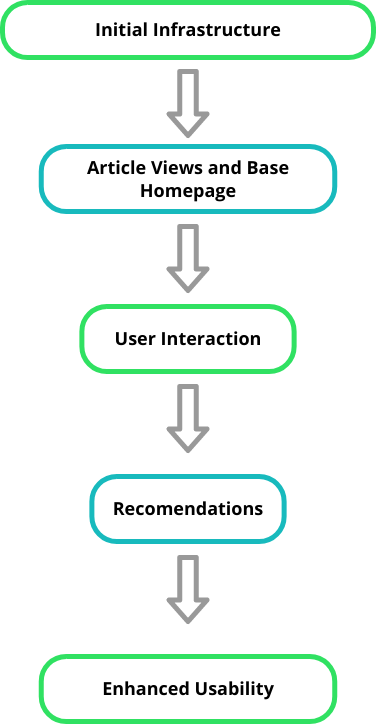
\includegraphics[width=0.3\linewidth]{roadmap.png}
    \caption{Roadmap des Projektes}
    \label{fig:roadmap}
\end{figure}

% Über den einzelnen Sprint Zielen gab es PIs
% das Konzept PIs kommen aus Safe und wurde hier als orrientierungshilfe für die Sprintziele verwendet

% Erklärung zu den unterschiedlichen PIs

\section{Einbringen von Sonstigen Aufgaben}
% Parallel zu PI, Mockups immer ein Product increment im vorraus
% Dokumentation immer ein PI hinterher